% Generated by refresh_charts.py from audited result snapshots.
\expandafter\def\csname tpp:OneSampleADE\endcsname{0.857}
\expandafter\def\csname tpp:BudgetReduction\endcsname{62}
\expandafter\def\csname tpp:ETHMin\endcsname{0.600}
\expandafter\def\csname tpp:ZaraTwoMin\endcsname{0.222}
\expandafter\def\csname tpp:MaxSeedSD\endcsname{0.023}
\expandafter\def\csname tpp:NoiseDominantFolds\endcsname{5}
\expandafter\def\csname tpp:UnivRuntime\endcsname{153.7}
\expandafter\def\csname tpp:UnivPreprocess\endcsname{143.6}

\providecommand{\TppInsight}[1]{\csname tpp:#1\endcsname}
\subsection{Trajectron++}
\label{sec:trajectronpp}
{\small\sffamily\color{Muted}LI Junhao \enspace / \enspace Pedestrian-only implementation \enspace / \enspace 15 audited runs}

\textbf{Forecasting mechanism and input audit.}
A recurrent graph encoder combines the target history and pedestrian
neighbors within 3\,m. A 25-category prior conditions the GRU decoder,
which samples and integrates correlated velocities
\cite{salzmann2020trajectron}. This variant uses one pedestrian edge type and
a hard radius mask. To prevent look-ahead through whole-track derivatives,
the adapter computes backward differences within the observed window.
Changing future target or neighbor positions leaves fixed-seed predictions
identical in all six conditions.

\textbf{More samples improve coverage.}
Re-scoring prefixes of the same forecast stream lowers minADE by
\TppInsight{BudgetReduction}\% from \TppInsight{OneSampleADE}\,m at \(K=1\)
to \ModelMetric{trajectronpp}{clean_0}{min_ade_mean}\,m at \(K=20\).
MeanADE stays near \ModelMetric{trajectronpp}{clean_0}{mean_ade_mean}\,m.
The change comes from giving the oracle more paths to choose from.
The twenty-sample Energy Score is
\ModelMetric{trajectronpp}{clean_0}{energy_score_mean}\,m.
Scene variation also matters. MinADE is \TppInsight{ETHMin}\,m on ETH and
\TppInsight{ZaraTwoMin}\,m on Zara2, while the largest within-scene standard
deviation across the three seeds is \TppInsight{MaxSeedSD}\,m.

\begin{figure}[H]
\centering
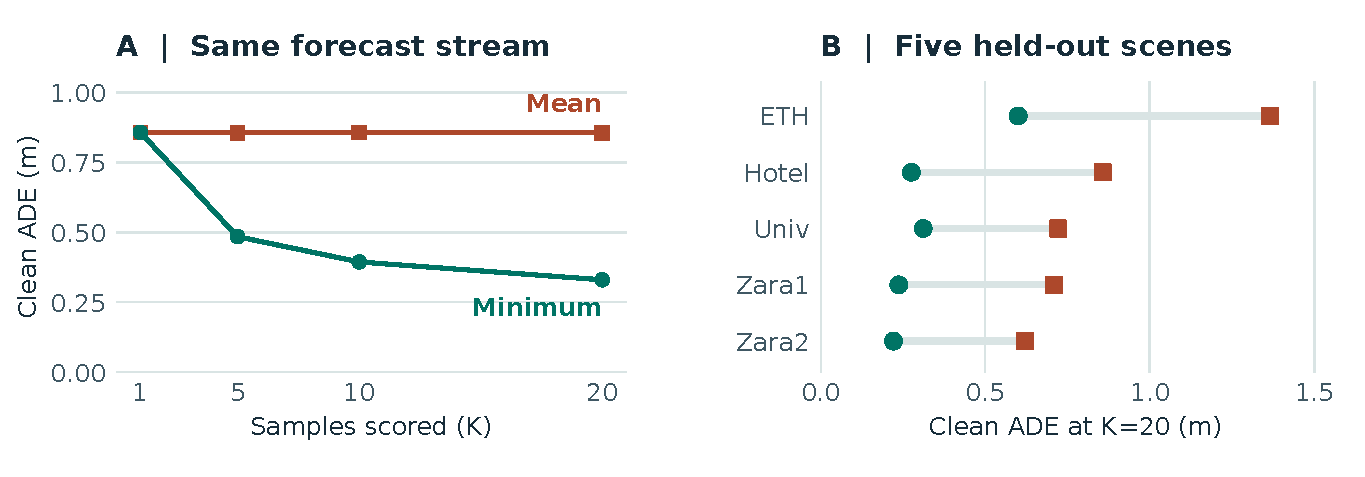
\includegraphics[width=\linewidth,height=1.73in,keepaspectratio]{contributions/trajectronpp/assets/sampling.pdf}
\caption{Clean forecast error. Panel A re-scores prefixes of the same
samples and weights the five holdouts equally. Panel B shows seed means
within each holdout at \(K=20\).}
\label{fig:trajectronpp-sampling}
\end{figure}

\textbf{Noise matters more than short gaps in this protocol.}
MeanADE increased by \ModelMeanADEChange{trajectronpp}{noise_020}\,m with
0.20\,m noise, versus \ModelMeanADEChange{trajectronpp}{missing_2}\,m with
two missing observations. Even 0.05\,m noise hurt more than missing two
in \TppInsight{NoiseDominantFolds} of five folds. Hotel's missing-two error
fell slightly, illustrating why the paired fold results matter alongside
the macro. Backward differences can amplify high-frequency position noise,
while the missing-suffix rule supplies a constant-velocity continuation.
Those mechanisms are consistent with the pattern. These runs do not isolate
their contributions.

\begin{figure}[H]
\centering
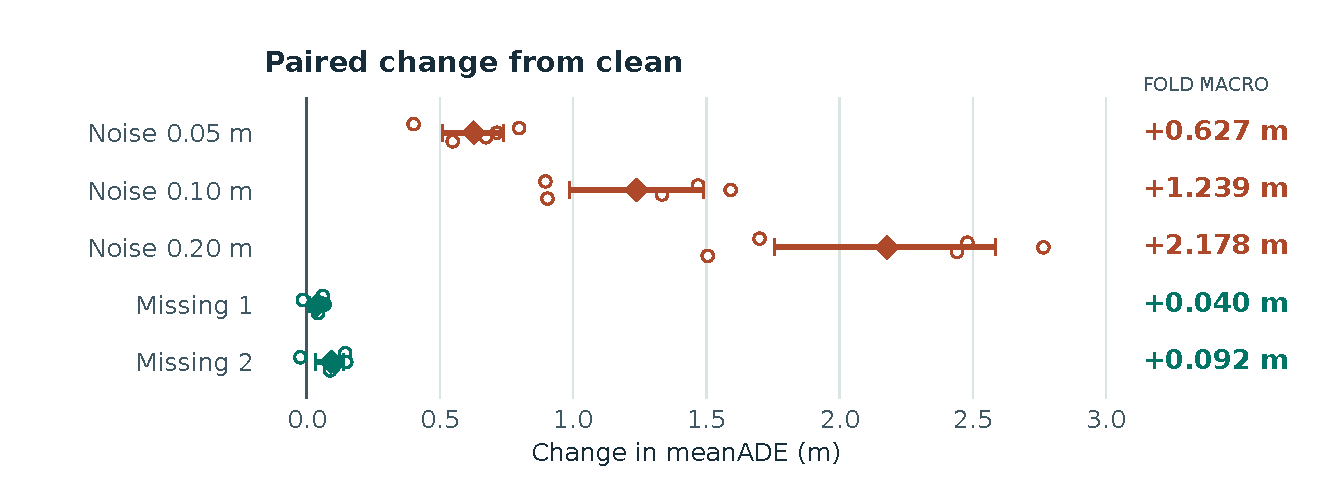
\includegraphics[width=\linewidth,height=1.73in,keepaspectratio]{contributions/trajectronpp/assets/paired_robustness.pdf}
\caption{MeanADE changes paired to clean within each holdout after averaging
seeds. Open circles are individual holdouts. Filled diamonds are equal-weight
macros with descriptive 95\% scene-bootstrap intervals across five holdouts.
Neighbor histories and future labels stay fixed.}
\label{fig:trajectronpp-robustness}
\end{figure}

\textbf{Where runtime goes.}
The median of run medians is \ModelRuntime{trajectronpp}{end_to_end_ms}\,ms
per 128 targets, with \ModelRuntime{trajectronpp}{preprocessing_ms}\,ms for
preprocessing and \ModelRuntime{trajectronpp}{prediction_sampling_ms}\,ms
for inference and sampling measured separately. Univ's median end-to-end
latency is \TppInsight{UnivRuntime}\,ms and preprocessing alone is
\TppInsight{UnivPreprocess}\,ms. A fixed target count still allows different
scene workloads. Use matched windows and stage boundaries when comparing
model efficiency.
